\documentclass[tikz,border=12pt]{standalone}

\usepackage[T1]{fontenc}
\usepackage{lmodern}
\usepackage{amsmath}
\usetikzlibrary{
  arrows.meta,
  backgrounds,
  fit,
  positioning,
  shadows.blur
}

\definecolor{pjBlue}{HTML}{2F6FED}
\definecolor{pjCyan}{HTML}{22A6B3}
\definecolor{pjGreen}{HTML}{2EAD70}
\definecolor{pjOrange}{HTML}{F28C28}
\definecolor{pjRed}{HTML}{D64545}
\definecolor{pjInk}{HTML}{1F2937}
\definecolor{pjMuted}{HTML}{6B7280}
\definecolor{pjPanel}{HTML}{F7F9FC}
\definecolor{pjLine}{HTML}{CBD5E1}

\tikzset{
  font=\sffamily,
  title/.style={font=\Large\bfseries\sffamily, text=pjInk},
  section/.style={font=\bfseries\sffamily, text=pjInk},
  note/.style={font=\scriptsize\sffamily, text=pjMuted, align=center},
  block/.style={
    draw=pjLine,
    very thick,
    rounded corners=4pt,
    fill=white,
    blur shadow={shadow blur steps=4, shadow opacity=14},
    align=center,
    minimum height=1.05cm,
    text=pjInk
  },
  data/.style={block, fill=pjBlue!7, draw=pjBlue!40},
  encoder/.style={block, fill=pjCyan!8, draw=pjCyan!55},
  latent/.style={block, fill=pjGreen!8, draw=pjGreen!55},
  predictor/.style={block, fill=pjOrange!10, draw=pjOrange!60},
  loss/.style={block, fill=pjRed!7, draw=pjRed!55},
  probe/.style={block, fill=pjMuted!8, draw=pjMuted!50, dashed},
  panel/.style={
    draw=pjLine,
    rounded corners=7pt,
    fill=pjPanel,
    inner sep=11pt
  },
  arrow/.style={-{Latex[length=3mm]}, very thick, draw=pjInk},
  softarrow/.style={-{Latex[length=2.6mm]}, thick, draw=pjMuted},
  dashedarrow/.style={-{Latex[length=2.6mm]}, thick, draw=pjMuted, dashed}
}

\begin{document}
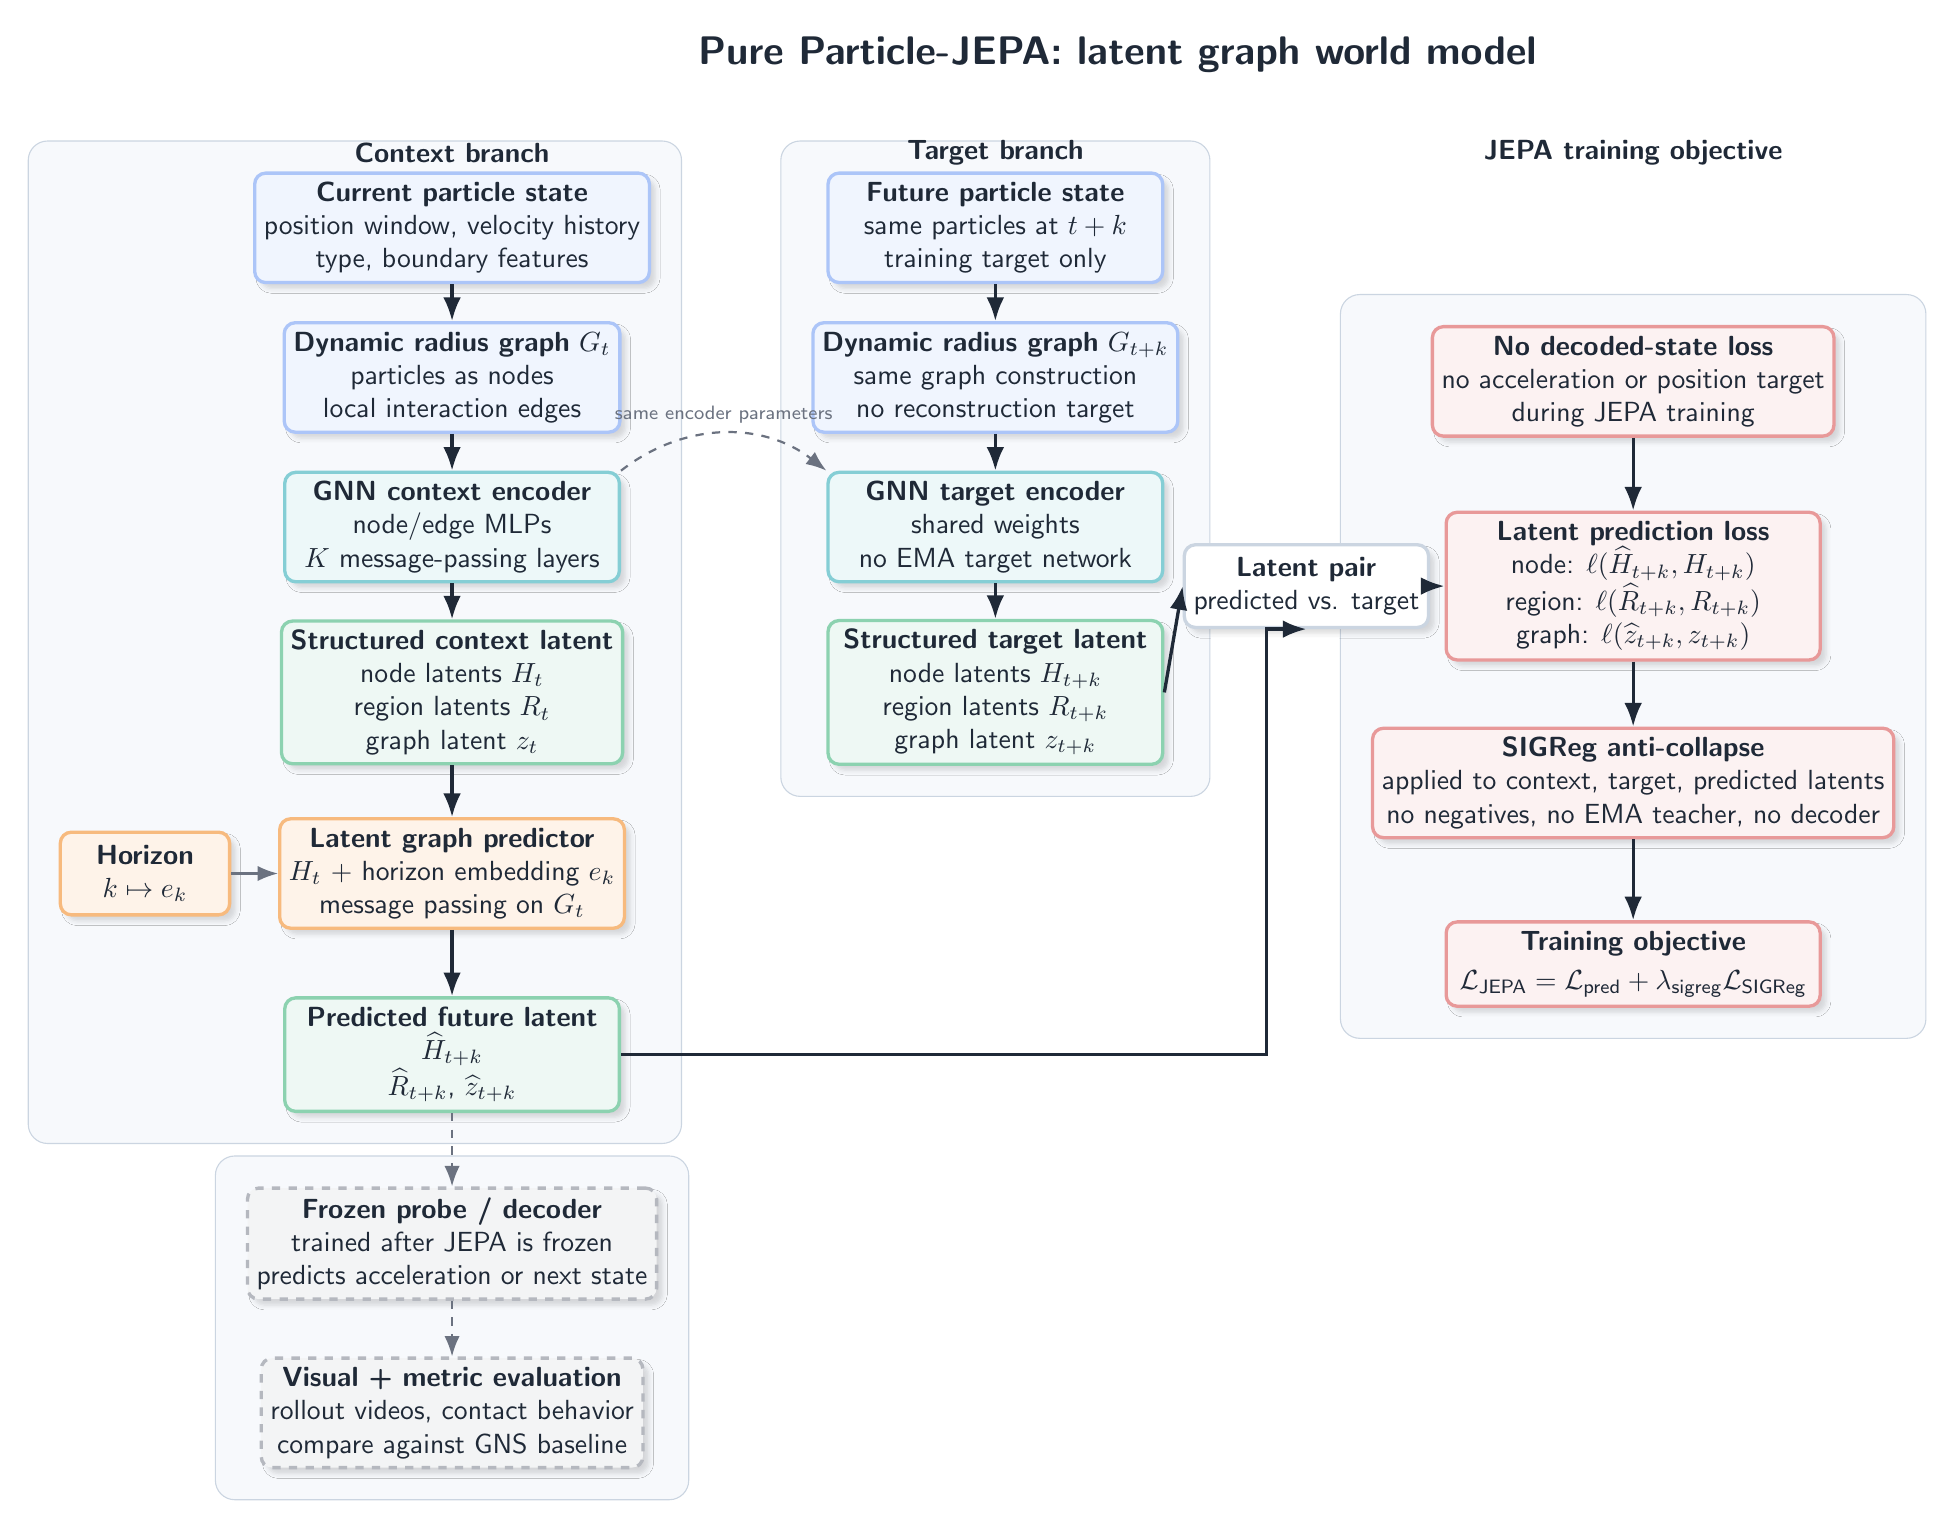
\begin{tikzpicture}[x=1cm,y=1cm]

% --------------------------------------------------------------------------
% Coordinates
% --------------------------------------------------------------------------
\node[title] at (8.45, 2.2) {Pure Particle-JEPA: latent graph world model};

\node[section] at (0, 0.95) {Context branch};
\node[section] at (6.9, 0.95) {Target branch};
\node[section] at (15.0, 0.95) {JEPA training objective};

% --------------------------------------------------------------------------
% Context branch
% --------------------------------------------------------------------------
\node[data, minimum width=4.25cm] (state_t) at (0,0) {
  \textbf{Current particle state}\\
  position window, velocity history\\
  type, boundary features
};

\node[data, minimum width=4.25cm] (graph_t) at (0,-1.9) {
  \textbf{Dynamic radius graph} $G_t$\\
  particles as nodes\\
  local interaction edges
};

\node[encoder, minimum width=4.25cm] (enc_t) at (0,-3.8) {
  \textbf{GNN context encoder}\\
  node/edge MLPs\\
  $K$ message-passing layers
};

\node[latent, minimum width=4.25cm] (lat_t) at (0,-5.9) {
  \textbf{Structured context latent}\\
  node latents $H_t$\\
  region latents $R_t$\\
  graph latent $z_t$
};

\node[predictor, minimum width=4.25cm] (pred) at (0,-8.2) {
  \textbf{Latent graph predictor}\\
  $H_t$ + horizon embedding $e_k$\\
  message passing on $G_t$
};

\node[latent, minimum width=4.25cm] (lat_pred) at (0,-10.5) {
  \textbf{Predicted future latent}\\
  $\widehat{H}_{t+k}$\\
  $\widehat{R}_{t+k}$, $\widehat{z}_{t+k}$
};

\node[predictor, minimum width=2.15cm] (horizon) at (-3.9,-8.2) {
  \textbf{Horizon}\\
  $k \mapsto e_k$
};

\draw[arrow] (state_t) -- (graph_t);
\draw[arrow] (graph_t) -- (enc_t);
\draw[arrow] (enc_t) -- (lat_t);
\draw[arrow] (lat_t) -- (pred);
\draw[arrow] (pred) -- (lat_pred);
\draw[softarrow] (horizon) -- (pred);

% --------------------------------------------------------------------------
% Target branch
% --------------------------------------------------------------------------
\node[data, minimum width=4.25cm] (state_f) at (6.9,0) {
  \textbf{Future particle state}\\
  same particles at $t+k$\\
  training target only
};

\node[data, minimum width=4.25cm] (graph_f) at (6.9,-1.9) {
  \textbf{Dynamic radius graph} $G_{t+k}$\\
  same graph construction\\
  no reconstruction target
};

\node[encoder, minimum width=4.25cm] (enc_f) at (6.9,-3.8) {
  \textbf{GNN target encoder}\\
  shared weights\\
  no EMA target network
};

\node[latent, minimum width=4.25cm] (lat_f) at (6.9,-5.9) {
  \textbf{Structured target latent}\\
  node latents $H_{t+k}$\\
  region latents $R_{t+k}$\\
  graph latent $z_{t+k}$
};

\draw[arrow] (state_f) -- (graph_f);
\draw[arrow] (graph_f) -- (enc_f);
\draw[arrow] (enc_f) -- (lat_f);

\draw[dashedarrow]
  (enc_t.north east)
  to[out=38,in=142]
  node[note, above] {same encoder parameters}
  (enc_f.north west);

% --------------------------------------------------------------------------
% JEPA losses
% --------------------------------------------------------------------------
\node[block, fill=white, draw=pjLine, minimum width=2.65cm] (pair) at (10.85,-4.55) {
  \textbf{Latent pair}\\
  predicted vs. target
};

\node[loss, minimum width=4.75cm] (loss_pred) at (15.0,-4.55) {
  \textbf{Latent prediction loss}\\
  node: $\ell(\widehat{H}_{t+k}, H_{t+k})$\\
  region: $\ell(\widehat{R}_{t+k}, R_{t+k})$\\
  graph: $\ell(\widehat{z}_{t+k}, z_{t+k})$
};

\node[loss, minimum width=4.75cm] (sigreg) at (15.0,-7.05) {
  \textbf{SIGReg anti-collapse}\\
  applied to context, target, predicted latents\\
  no negatives, no EMA teacher, no decoder
};

\node[loss, minimum width=4.75cm] (objective) at (15.0,-9.35) {
  \textbf{Training objective}\\[2pt]
  $\mathcal{L}_{\text{JEPA}} =
  \mathcal{L}_{\text{pred}} +
  \lambda_{\text{sigreg}}\mathcal{L}_{\text{SIGReg}}$
};

\node[loss, minimum width=4.75cm] (no_decode) at (15.0,-1.95) {
  \textbf{No decoded-state loss}\\
  no acceleration or position target\\
  during JEPA training
};

\draw[arrow] (lat_f.east) -- (pair.west);
\draw[arrow] (lat_pred.east) -- ++(8.2,0) |- (pair.south);
\draw[arrow] (pair.east) -- (loss_pred.west);
\draw[arrow] (no_decode) -- (loss_pred);
\draw[arrow] (loss_pred) -- (sigreg);
\draw[arrow] (sigreg) -- (objective);

% --------------------------------------------------------------------------
% Evaluation probe
% --------------------------------------------------------------------------
\node[probe, minimum width=4.25cm] (probe) at (0,-12.9) {
  \textbf{Frozen probe / decoder}\\
  trained after JEPA is frozen\\
  predicts acceleration or next state
};

\node[probe, minimum width=4.25cm] (eval) at (0,-15.05) {
  \textbf{Visual + metric evaluation}\\
  rollout videos, contact behavior\\
  compare against GNS baseline
};

\draw[dashedarrow] (lat_pred) -- (probe);
\draw[dashedarrow] (probe) -- (eval);

% --------------------------------------------------------------------------
% Background panels
% --------------------------------------------------------------------------
\begin{scope}[on background layer]
  \node[panel, fit=(state_t)(graph_t)(enc_t)(lat_t)(pred)(lat_pred)(horizon)] {};
  \node[panel, fit=(state_f)(graph_f)(enc_f)(lat_f)] {};
  \node[panel, fit=(no_decode)(loss_pred)(sigreg)(objective)] {};
  \node[panel, fit=(probe)(eval)] {};
\end{scope}

\end{tikzpicture}
\end{document}
